% This document is a playground for testing new commands before inserting them
% into the .sty file

\documentclass{scrartcl}

\usepackage{lilyglyphs}

% Print some text in the emmentaler font. Works for the dynamic letters
% and the digits:
\newcommand{\lilyText}[1]{{\fontspec[Scale=1.4]{Emmentaler-11}{#1}}}

%%%%%%%%%%%%%%%%%%%%%%%%
% Numbers and Dynamics %
%%%%%%%%%%%%%%%%%%%%%%%%

%\newcommand{\lilyNumber}[2][1.35]{\lilyText[#1]{#2}}

% general \time n/m command (prints time signature as a fraction in emmentaler font)
\newcommand*{\lilyTimeSignature}[2]{$\frac{\mbox{\lilyText{#1}}}{\mbox{\lilyText{#2}}}$}

\begin{document}
\section*{Time Signatures}
	\lilyText{sffpzm1+2}
	
	This is a normal Time signature: \lilyTimeSignature{3}{4}.
	
	As the plus sign is also directly accessible you can even
	write \lilyTimeSignature{3\,+\,7}{8+4} easily :-)

	%\lilyNumber
	
\section*{PGF/tikz}

Absatz, zusammen mit einem Notenkopf: 
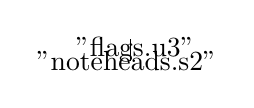
\begin{tikzpicture}
	\draw (0,0) node {\lilyGlyph{"noteheads.s2"}};
	\draw[semithick] (0.3ex,0) -- (0.3ex,0.8em);
	\draw (0.7ex,1ex) node {\lilyGlyph{"flags.u3"}};
\end{tikzpicture}

\Large
Neuer Absatz, zusammen mit einem Notenkopf: 
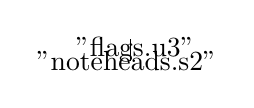
\begin{tikzpicture}
	\draw (0,0) node {\lilyGlyph{"noteheads.s2"}};
	\draw[semithick] (0.3ex,0) -- (0.3ex,0.8em);
	\draw (0.7ex,1ex) node {\lilyGlyph{"flags.u3"}};
\end{tikzpicture}

\normalsize
Neuer Absatz, zusammen mit einem Notenkopf: 
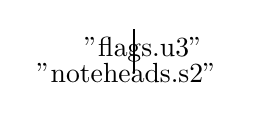
\begin{tikzpicture}[scale=2]
	\draw (0,0) node {\lilyGlyph{"noteheads.s2"}};
	\draw[semithick] (0.3ex,0) -- (0.3ex,0.8em);
	\draw (0.7ex,1ex) node {\lilyGlyph{"flags.u3"}};
\end{tikzpicture}

One sees: It is principally possible to combine graphical and textual elements with pgf/tikz,
but we definitely have to work on it some more: Especially it isn't scalable so far (explicitely or implicitely following text size)
\end{document}